\documentclass{beamer}
\usetheme{Singapore}
\usepackage{changepage}

%\usepackage{pstricks,pst-node,pst-tree}
\usepackage{amssymb,latexsym}
\usepackage{tikz}
\usepackage{graphicx}
\usepackage{fancyvrb}
\usepackage{hyperref}
\usepackage{fancybox}
\usepackage[listings]{tcolorbox}

\definecolor{codegreen}{rgb}{0,0.6,0}
\definecolor{codegray}{rgb}{0.5,0.5,0.5}
\definecolor{codepurple}{rgb}{0.58,0,0.82}
\definecolor{backcolour}{rgb}{0.95,0.95,0.92}

\lstdefinestyle{mystyle}{
    language=Python,
    backgroundcolor=\color{backcolour},   
    commentstyle=\color{codegreen},
    keywordstyle=\color{magenta},
    numberstyle=\tiny\color{codegray},
    stringstyle=\color{codepurple},
    basicstyle=\ttfamily\scriptsize,
    breakatwhitespace=false,         
    breaklines=true,                 
    captionpos=b,                    
    keepspaces=true,                 
    numbers=left,                    
    numbersep=5pt,                  
    showspaces=false,                
    showstringspaces=false,
    showtabs=false,                  
    tabsize=2,
    escapechar=|,
    frame=single
}

\lstset{style=mystyle}


\newcommand{\bi}{\begin{itemize}}
\newcommand{\li}{\item}
\newcommand{\ei}{\end{itemize}}
\newcommand{\Show}[1]{
\begin{center}
\shadowbox{\begin{minipage}{0.8\textwidth}
          #1
          \end{minipage}}
\end{center}
}
\newcommand{\arrow}{\ensuremath{\rightarrow}}

\newcommand{\uparr}{\ensuremath{\uparrow}}


\newcommand{\fig}[2]{\centerline{\includegraphics[width=#1\textwidth]{#2}}}

\newcommand{\bfr}[1]{\begin{frame}[fragile]\frametitle{{ #1 }}}
\newcommand{\efr}{\end{frame}}

\newcommand{\cola}{\begin{columns}\begin{column}{0.5\textwidth}}
\newcommand{\colb}{\end{column}\begin{column}{0.5\textwidth}}
\newcommand{\colc}{\end{column}\end{columns}}


\title{Programming Languages, Introduction}
\author{CSCI 312, Winter 2023}

\begin{document}

\begin{frame}
\maketitle
\end{frame}

\bfr{``The Perils of JavaSchools,'' \em Joel Spolsky}

\vfill

\centerline{
\shadowbox{
\parbox{3.5in}
{\large I have never met anyone who can do Scheme, Haskell, and C pointers
who can't pick up Java in two days, and create better Java code than
people with five years of experience in Java, but try explaining that
to the average HR drone.  }}}

\vfill
\end{frame}

\bfr{New languages are everywhere:}


Java, PHP,  Perl,  Python,  TCL,  Javascript, C\#,  Rust, Go, Zig, ...

Scripting languages for games, spreadsheets, editors ...

Data description languages for HTML, typesetting,
spreadsheets, music, graphics ...

\end{frame}

\bfr{Modeling Languages}

Learning a new programming languages means learning:
\bi
\li a peculiar syntax for the language,
\li behavior associated with each syntax,
\li numerous useful libraries, and
\li a collection of idioms that programmers of that language use.
\ei

\end{frame}


\bfr{Syntax doesn't tell us about a program's \em behavior}
Which two of these are most similar?
\begin{enumerate}
\item \lstinline{a [25]}
\item \lstinline{(vector-ref a 25)}
\item \lstinline{a [25]}
\item \lstinline{a [25]}
\end{enumerate}
\pause
The first and the second, obviously!
\bi
\li The first is in Python; it's an array reference and will signal an error
if the vector has less than 25 entries.

\li The second is in Scheme; it's an array reference and will signal an error
if the vector has less than 25 entries.

\li The third is in C; God help you if the array isn't big enough.

\li The fourth is in Haskell; it's a function applied to a list.
\ei

\end{frame}

\bfr{Syntax Matters}

\bi
\li Syntax is important:
\li Bad syntax can hide errors (Fortran).
\li Good syntax is easy to read and understand.
\li Good syntax makes it easy to express your ideas.
\li Try doing long division with Roman numerals sometime.
\ei

\end{frame}
\bfr{Syntax Matters, but not here}


\bi
\li Syntax is irrelevant to semantics.
\li We're interested in semantics.
\li Programs are trees, not strings, anyway.
\ei


\begin{lstlisting}
((2**3)/sqrt(x))/(5 - 2x)+3
\end{lstlisting}
\footnotesize
\begin{lstlisting}
Add(
  Div(
    Div(
      Exp(Num(2), Num(3))
      Call(Name(sqrt), Args([Name(x)])
    )
    Sub(Num(5), Mul(Num(2), Name(x)))
  )
  Num(3)
)
\end{lstlisting} 

\end{frame}

\bfr{Parsing in Python}
\bi
\li
Python has a builtin module \lstinline{ast} that provides access to 
Python parser tools.
\li
I have written some convenience tools in \lstinline{ast_utilities.py}.
\ei

\begin{lstlisting}
>>> from ast import parse, dump
>>> from ast_utilities import *
>>> parse('x=x+1')
<_ast.Module object at 0x0000022032093308>
>>> dump(parse('x=x+1'))
"Module(body=[Assign(targets=[Name(id='x', ctx=Store())], value=BinOp(left=Name(id='x', ctx=Load()), op=Add(), right=Num(n=1)))])"
\end{lstlisting}  

\end{frame}

\bfr{Pretty-printed Python Parses}
\cola
\begin{lstlisting}
>>> ppp('x=x+1',pruning=False)
x=x+1
Module(
  body=[
    Assign(
      targets=[
        Name(
          id='x',
          ctx=Store(
            ))],
      value=BinOp(
        left=Name(
          id='x',
          ctx=Load(
            )),
        op=Add(
          ),
        right=Num(
          n=1)))])
\end{lstlisting}  
\colb
With tree pruning:
\begin{lstlisting}
>>> ppp('x=x+1')
x=x+1
Module(
  body=[
    Assign(
      targets=[
        Name(
          id='x')],
      value=BinOp(
        left=Name(
          id='x'),
        op=Add(
          ),
        right=Num(
          n=1)))])
\end{lstlisting}  
\begin{lstlisting}
class Module: ...
class Assign: ...
class BinOp: ...
\end{lstlisting}
\colc 

\end{frame}

\bfr{{\tt prune}: an example of processing an AST}
Dispatching on type, recursion through subtrees:
\begin{lstlisting}
def prune(tree):
    if type(tree) is Module:
        return Module(body=prune(tree.body))
    elif type(tree) is list:
        return [prune(x) for x in tree]
    elif type(tree) is Name:
        return Name(id=tree.id)
    elif type(tree) is BinOp:
        return BinOp(left=prune(tree.left),
                     op=tree.op,
                     right=prune(tree.right))
    ...
    else:
        return tree
\end{lstlisting}  

\end{frame}

\bfr{Exploring Python Parse Trees}
\begin{lstlisting}
>>> dump(parse('x'))
"Module(body=[Expr(value=Name(id='x', ctx=Load()))])"
>>> ppp('x')
x
Module(
  body=[
    Expr(
      value=Name(
        id='x'))])
------------------------------------------------------------
>>> dump(parse('x').body[0])
"Expr(value=Name(id='x', ctx=Load()))"
>>> ppd(parse('x').body[0])
Expr(
  value=Name(
    id='x'))
------------------------------------------------------------
\end{lstlisting}  

\end{frame}

\bfr{Homework \# 1}
Use Python parse trees to translate arithmetic expressions
into prefix, postfix, and fully parenthsized infix forms.

Also build a calculator!


\begin{lstlisting}
>>> s = '13+4**(5+6)/7'
>>> prefix(s)
'+ 13 / ** 4 + 5 6 7'
>>> postfix(s)
'13 4 5 6 + ** 7 / +'
>>> infix(s)
'(13+((4**(5+6))/7))'
>>> calc(s)
599199.2857142857
>>> eval(s)
599199.2857142857
\end{lstlisting}  

\end{frame}
\bfr{Finish the unit test as well}
\begin{lstlisting}
import unittest
from ast_homework import *

class ast_Test(unittest.TestCase):
    def test_ast_calc(self):
        self.assertAlmostEqual(calc('9 + 3 * 4 / 2'),
                                    9 + 3 * 4 / 2)
        self.assertAlmostEqual(calc('13+4**(5+6)/7'),
                                    13+4**(5+6)/7)

    def test_ast_postfix(self):
        self.assertEqual(postfix('2+3+4'),
                         '2 3 + 4 +')


if __name__ == '__main__':
    unittest.main()
\end{lstlisting}  

\end{frame}

\bfr{In this course:  trees and their semantics}

\bi
\li How do we express semantics?
\li English (natural language) is notoriously sloppy.
\li Mathematics is difficult and abstract:
\bi\li denotational semantics\li operational semantics
\li axiomatic semantics\ei
\li We will use {\bf interpreter semantics}:
\\ to explain a language, build an interpreter for it.
\ei
\end{frame}

\bfr{Interpreting language {\em vs.} interpreted language}

\begin{center}
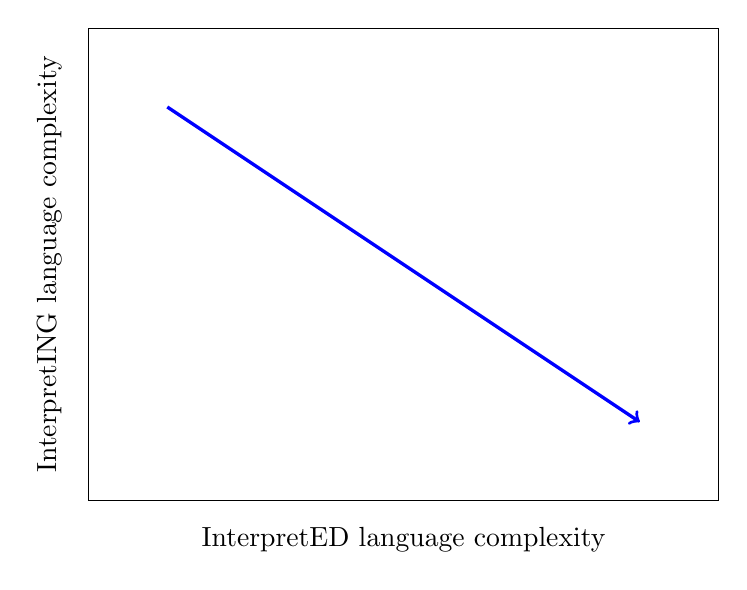
\begin{tikzpicture}
\draw (0,0) -- (8,0) -- (8,6) -- (0,6) -- cycle;
\draw[arrows=->,color=blue,very thick] (1,5) -- (7,1);
\draw (4,-0.5) node {InterpretED language complexity};
\draw (-0.5,3) node[rotate=90] {InterpretING language complexity};
\end{tikzpicture}

\end{center}

\end{frame}

\bfr{Our InterpretING Language: Scheme}

\bi
\li \url{https://racket-lang.org/}
\bi\li Our implementation \ei
\li \url{https://docs.racket-lang.org/index.html}
\bi\li Work through the {\em Quick} tutorial\ei
\li Also do one or more of the following:
\bi
\li \url{https://ds26gte.github.io/tyscheme/}
\bi\li Work through Chapters 1 to 6: Recursion
\li Note that we use Racket instead of mzscheme\ei
\li \url{https://www.scheme.com/tspl4/}
\bi\li Work through Chapters 1 and 2 
\li Note that we use Racket instead of chez scheme\ei
\li \url{https://htdp.org/}
\bi\li Very careful exposition.\ei
\ei\ei

\end{frame}
\end{document}
